\subsection{Lessons Learned and Training Dynamics}
\label{subsec:lessons_learned}

Evaluating model convergence across all training configurations reveals clear patterns regarding spatial regularization, overfitting control, and class dependent feature learning. Complete training histories for both Cat and Dog datasets across all task configurations are provided in Appendix \ref{sec:appendix_curves}.

\subsubsection{Generalization and Overfitting Without Regularization}
Training from uninitialized weights without spatial data transforms leads to rapid memorization. In the unregularized baseline run (Task 7), training accuracy steadily progressed past $87\%$ for dogs and $58\%$ for cats. However, validation loss reached its global minimum early (epoch 65 for dogs, epoch 40 for cats) before drifting upwards. Final validation accuracy capped at $78.66\%$ for dogs and $46.13\%$ for cats. Without regularizing transformations, convolutional layers optimize for static background artifacts rather than generalized foreground patterns.
\begin{figure}[t!]
    \centering
    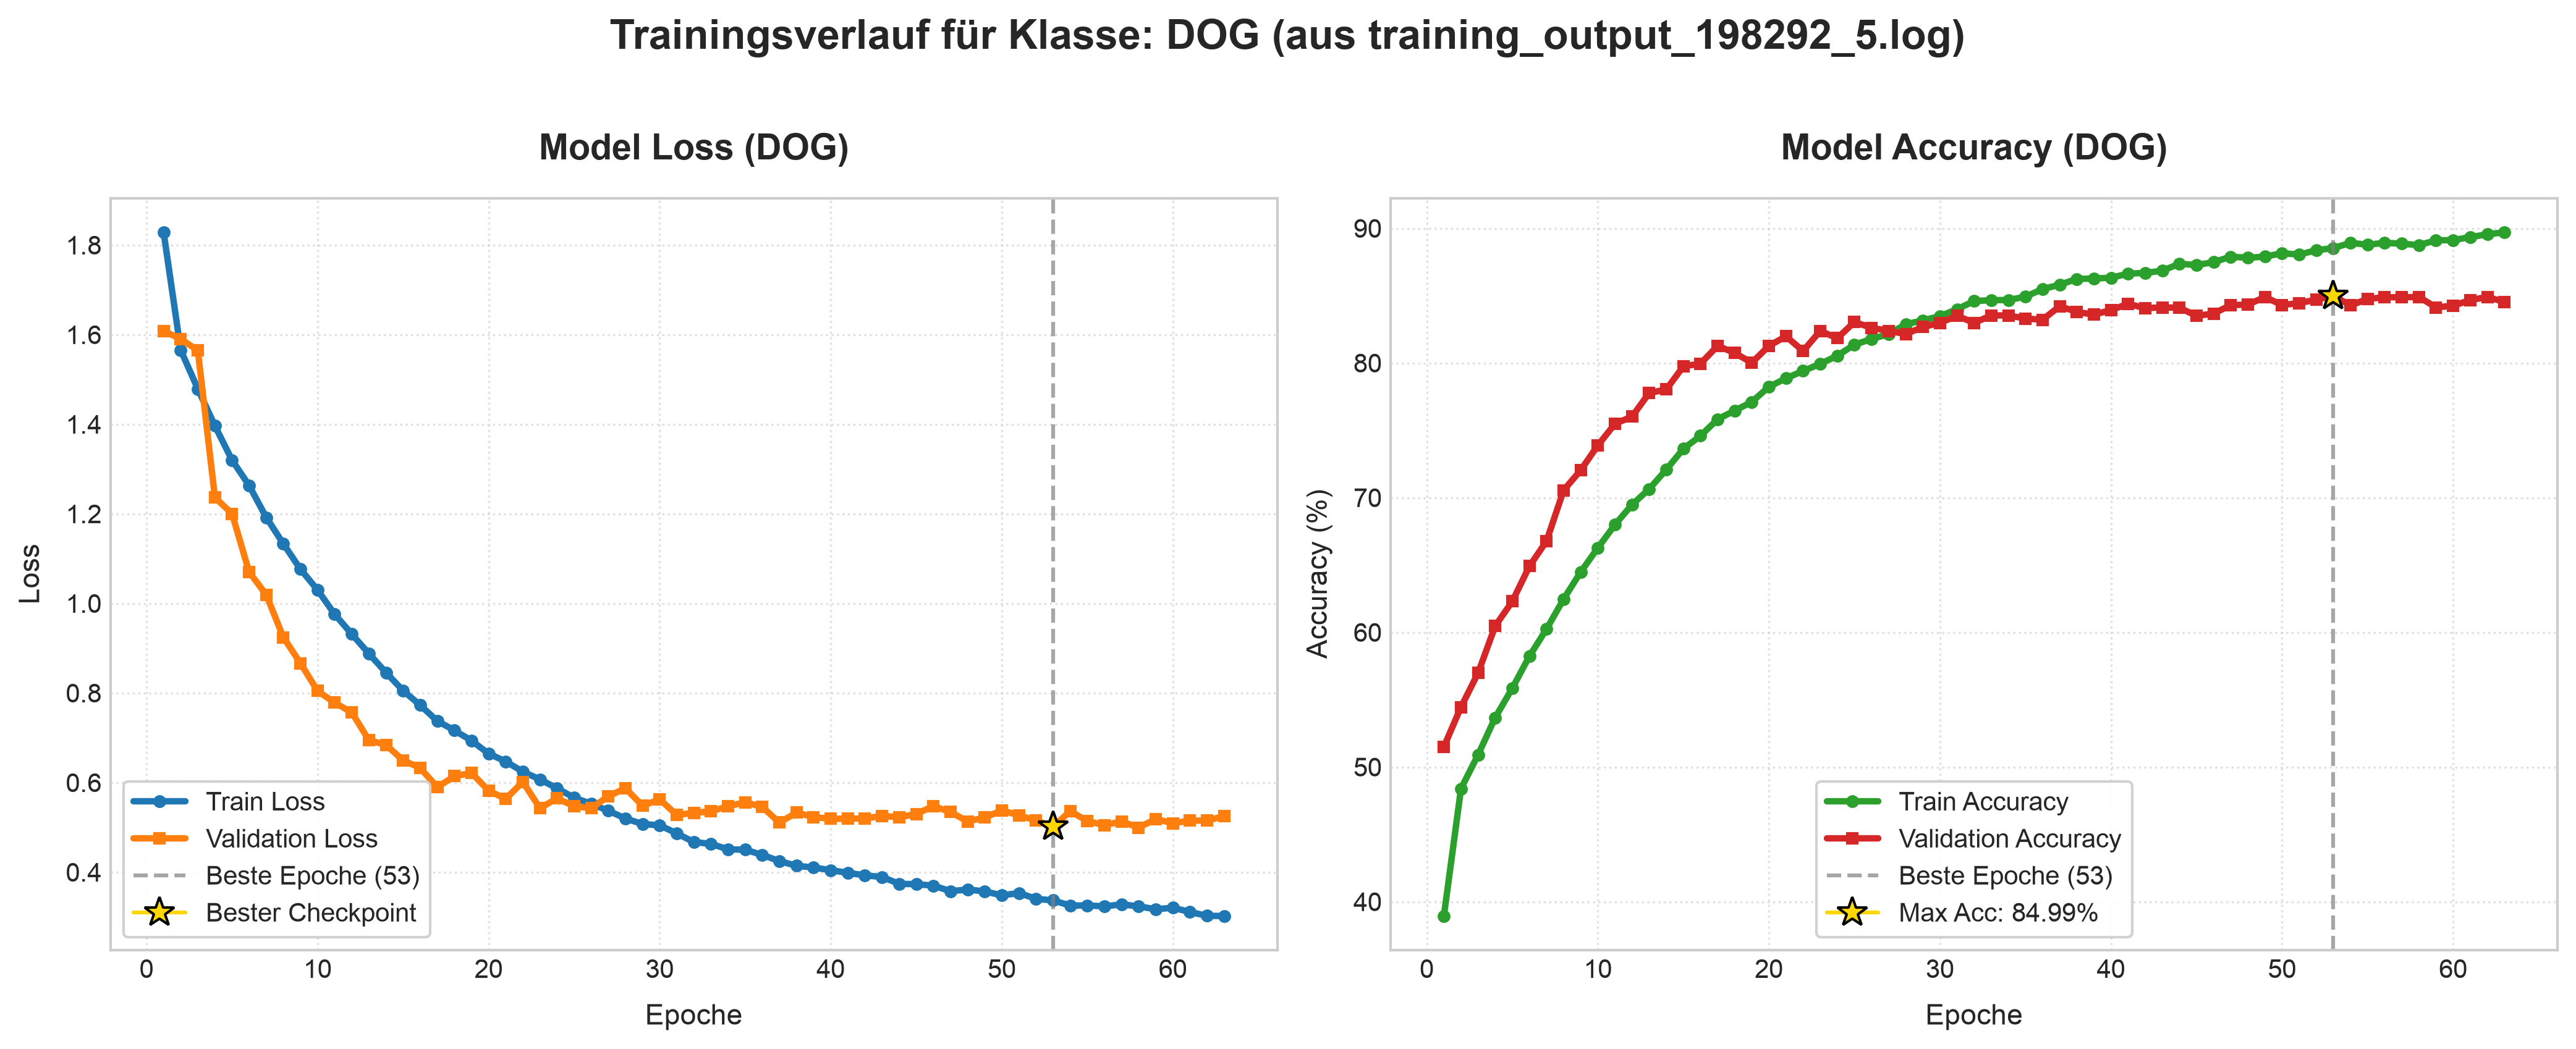
\includegraphics[width=\columnwidth]{../L_A_Graphs/training_output_198292_5_dog.png}
    \caption{Training and validation progression for the top performing CropMix configuration (Task 5). The validation loss curve remains stable across 50 epochs, effectively preventing premature overfitting.}
    \label{fig:best_run_cropmix}
\end{figure}

\subsubsection{Augmentation Efficacy and the Impact of CropMix}
Applying targeted image transformations significantly improves generalization across both sub datasets:
\begin{itemize}
    \item \textbf{Gaussian Blur (Task 3):} Attenuates high frequency texture noise, elevating validation accuracy to $82.96\%$ for dogs and $47.13\%$ for cats.
    \item \textbf{Horizontal Mirroring (Task 4):} Enforces spatial invariance, pushing validation accuracy to $84.47\%$ for dogs and $49.89\%$ for cats.
    \item \textbf{CropMix (Task 5):} Mixing image regions acts as a strong spatial regularizer. For dogs, CropMix increases validation accuracy to $84.99\%$ while completely flattening the validation loss curve over 50 epochs.
    \item \textbf{Combined Transformations (Task 6):} Applying all transformations simultaneously yields $85.02\%$ accuracy on dogs.
\end{itemize}

Comparing Task 5 ($84.99\%$) with Task 6 ($85.02\%$) demonstrates that CropMix accounts for virtually all performance improvements on the dog classification task, making additional filters like blurring largely redundant.
\subsubsection{Augmentation Efficacy and the Impact of CropMix}
Applying targeted image transformations significantly improves generalization across both sub datasets:
\begin{itemize}
    \item \textbf{Gaussian Blur (Task 3):} Attenuates high frequency texture noise, elevating validation accuracy to $82.96\%$ for dogs and $47.13\%$ for cats.
    \item \textbf{Horizontal Mirroring (Task 4):} Enforces spatial invariance, pushing validation accuracy to $84.47\%$ for dogs and $49.89\%$ for cats.
    \item \textbf{CropMix (Task 5):} Mixing image regions acts as a strong spatial regularizer. As illustrated in Figure \ref{fig:best_run_cropmix}, CropMix increases validation accuracy to $84.99\%$ for dogs while completely flattening the validation loss curve over 50 epochs.
    \item \textbf{Combined Transformations (Task 6):} Applying all transformations simultaneously yields $85.02\%$ accuracy on dogs.
\end{itemize}

\subsubsection{Domain Complexity Disparity Between Cats and Dogs}
Across every single training configuration, a persistent performance gap exists between dog classification ($78.66\%$ to $85.02\%$) and cat classification ($41.51\%$ to $49.89\%$). This disparity stems from underlying feature distributions:
\begin{itemize}
    \item \textbf{Dog Breeds:} Present large morphological variations in body proportions, muzzle shape, and coat color, yielding high inter class variance that CNN backbones isolate easily.
    \item \textbf{Cat Breeds:} Feature subtle, fine grained visual similarities with minimal structural variation. Standard cross entropy loss without dedicated fine grained feature extraction struggles to separate these classes when training from scratch.
\end{itemize}

\subsubsection{Key Practical Findings}
Our empirical evaluation yields three core findings for training vision backbones from scratch:
\begin{enumerate}
    \item Spatial patch mixing techniques like CropMix are the most effective regularizer, driving accuracy gains of over $6\%$ while preventing loss divergence.
    \item Early stopping based on validation loss minimums is critical when training without heavy spatial augmentation, as validation error degrades while training loss continues to fall \cite{prechelt1998early}.
    \item Feature difficulty varies significantly by domain; subtle fine grained structures (like cat breeds) require specialized architectural heads or pretraining rather than standard augmentation alone.
\end{enumerate}